\clearpage
\subsection{A worked example of an integer-energy tie}
Consider a Q3 block whose rows are Ir, K, La and Li and whose columns are Ge, Hf, Hg and In. We select this particular block by an explicit diagnostic rule: among the 169 Q3 blocks it has the largest spread of original scores tied at the lowest integer cost. It illustrates the cost of returning a single arbitrary ground state when the solver can return the whole tied set.

\begin{figure}[ht]
\centering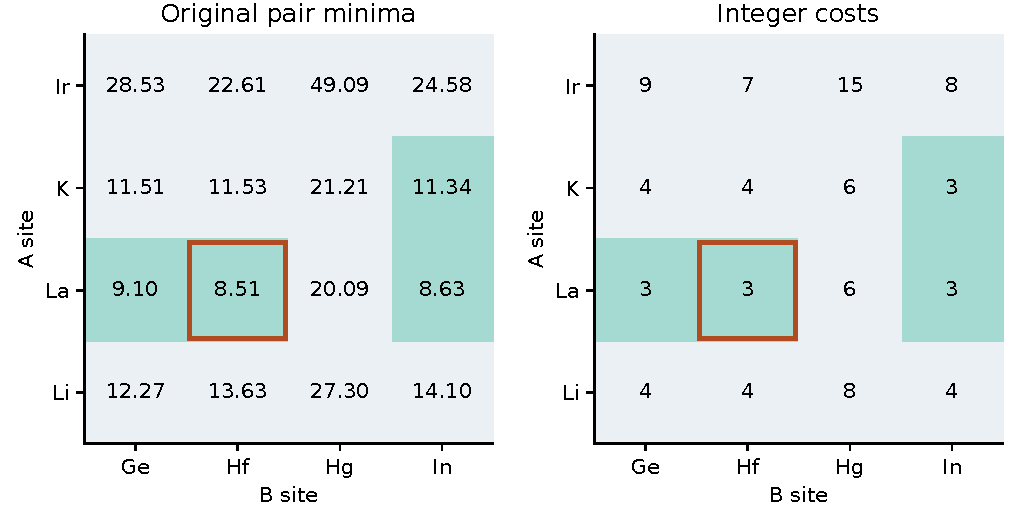
\includegraphics[width=.91\linewidth]{figures/tied_block.pdf}
\caption{The same Q3 block before and after Eq.~\eqref{eq:bins}. Green cells share the minimum integer cost. The outline marks the cell with the smallest original score. Displayed raw costs are rounded to two decimals after the calculation.}\label{fig:tile}
\end{figure}

The largest score in this block is 49.089358. The spacing of one integer bin is consequently about $49.089358/15=3.2726$ score units. Four pairs occupy the lowest bin. Their original scores are 8.511569 for La--Hf, 8.629274 for La--In, 9.102727 for La--Ge and 11.339649 for K--In. Each pair already carries its own minimizing $X$ from Eq.~\eqref{eq:envelope}. Selecting K--In would sacrifice 2.828081 units despite reaching the same minimum integer energy. Reading back the four original values returns La--Hf.

This example explains the difference between feasibility and selection accuracy. The penalty $P=16$ certifies one A and one B for every ground state in this block. It cannot distinguish the four green cells in Figure~\ref{fig:tile}. The monotonicity argument only places the best real-valued candidate somewhere among them. Full ground-state retrieval plus the original-score comparison is the additional condition needed for equality with the floating-point block minimum.

The distinction matters beyond this example. Multiple optimum pairs occur in 70 of 169 Q3 blocks and 71 of 169 Q2 blocks. The cost table in the next section includes time spent decoding and resolving those ties. These are within-block alternatives. Global selection still compares all 169 retained representatives using their original surrogate scores.

